\section{Relations} \label{S:relations}
\setcounter{previewactivity}{0}
%
\begin{previewactivity}[\textbf{The United States of America}] \label{PA:USA} \hfill \\
Recall from Section~\ref{S:cartesian} that the \textbf{Cartesian product}
\index{Cartesian product}%
 of two sets  $A$  and  $B$, written  $A \times B$, is the set of all ordered pairs  
$\left( {a,b} \right)$,  where  $a \in A$  and  $b \in B$.  That is,
$A \times B = \left\{ {\left( {a,b} \right)  \mid a \in A\text{ and }b \in B} \right\}$.

\noindent
Let  $A$  be the set of all states in the United States and let
\[
R = \left\{ { {\left( {x, y} \right) \in A \times A } \mid x \text{  and  }y 
\text{  have a land border in common}} \right\}\!.
\]
For example, since California and Oregon have a land border, we can say that 
$(\text{California, Oregon}) \in R$ and $(\text{Oregon, California}) \in R$.  Also, since California and Michigan do not share a land border, $\text{(California, Michigan)} \notin R$ and 
$(\text{Michigan, California}) \notin R$.
\begin{enumerate}
\item Use the roster method  to specify the elements in each of the following sets:
\begin{enumerate}
\item $B = \left\{ {y \in A\left| {\left( {\text{Michigan, }y} \right) \in R} \right.} \right\}$

\item $C = \left\{ {x \in A\left| {\left( {x,\text{Michigan}} \right) \in R} \right.} \right\}$

\item $D = \left\{ {y \in A\left| {\left( {\text{Wisconsin, }y} \right) \in R} \right.} \right\}$

\end{enumerate}

\item Find two different examples of two ordered pairs,  $\left( {x, y} \right)$ and 
$\left( {y, z} \right)$ such that  $\left( {x, y} \right) \in R$,  
$\left( {y, z} \right) \in R$,  but  $\left( {x, z} \right)\not  \in R$, or explain why no such example exists.  Based on this, is the following conditional statement true or false?
\begin{center}
For all $x, y, z \in A$, if $(x, y) \in R$ and $(y, z) \in R$, then $(x, z) \in R$.
\end{center}

\item Is the following conditional statement true or false?  Explain.
\begin{center}
For all $x, y \in A$, if $(x, y) \in R$, then $(y, x) \in R$.
\end{center}


%\item Are the following statements true or false?  Justify your conclusions.
%\begin{enumerate}
%\item For all $x, y \in A$, if $(x, y) \in R$, then $(y, x) \in R$.
%\item For all $x, y, z \in A$, if $(x, y) \in R$ and $(y, z) \in R$, then $(x, z) \in R$.
%\end{enumerate}

%\item In Section~\ref{S:inversefunctions}, we learned how to represent a function as a set of ordered pairs, and we learned under what conditions a set of ordered pairs can be used to define a function. Can the set  $R$  be used to define a function from the set  $A$  to the set  $A$?  Explain.
\end{enumerate}
\end{previewactivity}
\hbreak

\endinput

\begin{previewactivity}[\textbf{The Solution Set of an Equation with Two Variables}] \label{PA:eqn2variables} \hfill \\
In Section~\ref{S:predicates}, we introduced the concept of the \textbf{truth set of an open sentence with one variable}.
\index{truth set}%
  This was defined to be the set of all elements in the universal set that can be substituted for the variable to make the open sentence a true proposition.  Assume that  $x$  and  $y$  represent real numbers.  Then the equation
\[
4x^2  + y^2  = 16
\]
is an open sentence with two variables.  An element of the truth set of this open sentence (also called a solution of the equation) is an ordered pair  $\left( {a, b} \right)$ of real numbers so that when  $a$  is substituted for  $x$  and  $b$  is substituted for  $y$, the predicate becomes a true statement (a true equation in this case).  We can use set builder notation to describe the truth set $S$ of this equation with two variables as follows:
\[
S = \left\{ (x, y) \in \R \times \R \mid 4x^2 + y^2 = 16 \right\}\!.
\]
When a set is a truth set of an open sentence that is an equation, we also call the set the 
\textbf{solution set}
\index{solution set}%
 of the equation.
\begin{enumerate}
\item List four different elements of the set $S$\!.

\item The graph of the equation  $4x^2  + y^2  = 16$  in the $xy$-coordinate plane is an ellipse.  Draw the graph and explain why this graph is a representation of the truth set (solution set) of the equation $4x^2 + y^2 = 16$.

%\item Write a description of the solution set  $S$  of the equation  $x^2  + y^2  = 25$ using set builder notation.

%\pagebreak
\item Describe each of the following sets as an interval of real numbers:
\label{PA:eqn2variables3}
\begin{enumerate}
\item $A = \left\{ x \in \R \mid \text{ there exists a } y \in \R \text{ such that } 4x^2 + y^2 = 16 \right\}$.

\item $B = \left\{ y \in \R \mid \text{ there exists an } x \in \R \text{ such that } 4x^2 + y^2 = 16 \right\}$.
\end{enumerate}

\end{enumerate}
\end{previewactivity}
\hbreak
%

%\begin{previewactivity}[A Set of Order Pairs] \label{PA:orderedpairs} \hfill \\
%\noindent
%For another exampLet $\R^* = \left\{ y \in \R \mid y \geq 0 \right\}$ and let
%$F = \left\{ (x, y) \in \R \times \R^* \mid y = x^2 \right\}$.
%
%\begin{enumerate}
%\item List five different ordered pairs that are in the set $F$.
%
%\item Use the roster method to specify the elements of each of the following the sets:
%\begin{multicols}{2}
%\begin{enumerate}
%\item $A = \left\{ x \in \R \mid (x, 4) \in F \right\}$
%\item $B = \left\{ x \in \R \mid (x, 10) \in F \right\}$
%\item $C = \left\{ y \in \R^* \mid (5, y) \in F \right\}$
%\item $D = \left\{ y \in \R^* \mid (-3, y) \in F \right\}$
%\end{enumerate}
%\end{multicols}
%
%\item Can the set  $F$  be used to define a function from the set  $\R$  to the set  $\R^*$?  Explain.
%
%\end{enumerate}
%\end{previewactivity}
%\hbreak

\endinput

%%\begin{previewactivity}[The Telephone Keypad] \label{PA:telephone} \hfill
%
%The following diagram represents the keypad for a telephone.
%
%\begin{figure}[h]
%\begin{center}
%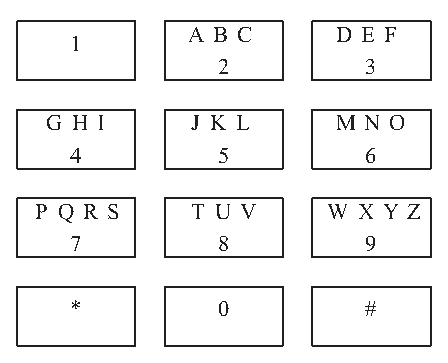
\includegraphics{figps-phone.eps}
%%\caption{Composition of Functions} \label{fig:functioncomposition2}
%\end{center}
%\end{figure}
%
%Let  $\Gamma  = \left\{ {0, 1, 2,  \ldots , 8, 9} \right\}$, and let  $\Delta $ be the set of all upper case letters in the English alphabet.  (\underline{Note}:  We are using the uppercase Greek letters gamma, $\Gamma $, and  delta, $\Delta $, to avoid confusion with the letters on the keypad.)  Define  $\Omega $, the uppercase Greek letter omega, to be the following subset of  
%$\Gamma  \times \Delta $:
%\[
%\Omega  = \left\{ { {\left( {x, y} \right) \in \Gamma  \times \Delta  } \mid x\text{  and  }y\text{  are on the same button}} \right\}.
%\]
%
%\begin{enumerate}
%\item Determine at least five different ordered pairs in  $\Gamma  \times \Delta $  that are elements of  $\Omega $.
%
%\item Determine at least five different ordered pairs in  $\Gamma  \times \Delta $  that are not elements of  $\Omega $.
%
%\item Determine all elements of the set  
%$\left\{ {\ {x \in \Gamma  } \mid \left( {\exists y \in \Delta } \right)\left( {\left( {x, y} \right) \in \Omega } \right)} \right\}$. \label{PA:telephone3}
%
%\item Determine all elements of the set  
%$\left\{ { {y \in \Delta  } \mid \left( {\exists x \in \Gamma } \right)\left( {\left( {x, y} \right) \in \Omega } \right)} \right\}$.  \label{PA:telephone4}
%\end{enumerate}
%\end{previewactivity}
%\hbreak
%

\begin{previewactivity}[The United States of America] \label{PA:USA} \hfill \\
Recall from Section~\ref{S:cartesian} that the \textbf{Cartesian product}
\index{Cartesian product}%
 of two sets  $A$  and  $B$, written  $A \times B$, is the set of all ordered pairs  
$\left( {a,b} \right)$,  where  $a \in A$  and  $b \in B$.  That is,
$A \times B = \left\{ {\left( {a,b} \right)  \mid a \in A\text{ and }b \in B} \right\}$.

\vskip6pt
Let  $A$  be the set of all states in the United States and let
\[
R = \left\{ { {\left( {x, y} \right) \in A \times A } \mid x \text{  and  }y 
\text{  have a land border in common}} \right\}\!.
\]
\begin{enumerate}
\item Use the roster method for defining a set to list all the elements in each of the following sets:
\begin{enumerate}
\item $A = \left\{ {y \in A\left| {\left( {\text{Michigan, }y} \right) \in R} \right.} \right\}$

\item $B = \left\{ {x \in A\left| {\left( {x,\text{Michigan}} \right) \in R} \right.} \right\}$

\item $C = \left\{ {y \in A\left| {\left( {\text{Wisconsin, }y} \right) \in R} \right.} \right\}$

\end{enumerate}

\item Find two different examples of two ordered pairs,  $\left( {x, y} \right)$ and 
$\left( {y, z} \right)$ such that  $\left( {x, y} \right) \in R$,  
$\left( {y, z} \right) \in R$,  but  $\left( {x, z} \right)\not  \in R$, or explain why no such example exists.

%\item Are the following statements true or false?  Justify your conclusions.
%\begin{enumerate}
%\item For all $x, y \in A$, if $(x, y) \in R$, then $(y, x) \in R$.
%\item For all $x, y, z \in A$, if $(x, y) \in R$ and $(y, z) \in R$, then $(x, z) \in R$.
%\end{enumerate}

\item In Section~\ref{S:inversefunctions}, we learned how to represent a function as a set of ordered pairs, and we learned under what conditions a set of ordered pairs can be used to define a function. Can the set  $R$  be used to define a function from the set  $A$  to the set  $A$?  Explain.
\end{enumerate}
\end{previewactivity}
\hbreak

\begin{previewactivity}[An Equation with Two Variables] \label{PA:eqn2variables} \hfill \\
In Section~\ref{S:predicates}, we introduced the concept of the \textbf{truth set of a predicate with one variable}.
\index{truth set}%
  This was defined to be the set of all elements in the universal set that can be substituted for the variable to make the predicate a true proposition.

Assume that  $x$  and  $y$  represent real numbers.  Then 

\[
4x^2  + y^2  = 16
\]
is a predicate with two variables.  An element of the truth set of this predicate (also called a solution of the equation) is an ordered pair  $\left( {a, b} \right)$ of real numbers so that when  $a$  is substituted for  $x$  and  $b$  is substituted for  $y$, the predicate becomes a true proposition (a true equation in this case).  We can use set builder notation to describe the truth set $S$ of this equation with two variables as follows:
\[
S = \left\{ (x, y) \in \R \times \R \mid 4x^2 + y^2 = 16 \right\}\!.
\]
When a set is a truth set of a predicate that is an equation, we also call the set the 
\textbf{solution set} of the equation.
\begin{enumerate}
\item List four different elements of the set $S$\!.

\item The graph of the equation  $4x^2  + y^2  = 16$  in the $xy$-coordinate plane is an ellipse.  Draw the graph and explain why this graph is a representation of the truth set (solutions set) of the equation $4x^2 + y^2 = 16$.

%\item Write a description of the solution set  $S$  of the equation  $x^2  + y^2  = 25$ using set builder notation.

%\pagebreak
\item Describe each of the following sets as an interval of real numbers:
\label{PA:eqn2variables3}
\begin{enumerate}
\item $A = \left\{ x \in \R \mid \text{ there exists a } y \in \R \text{ such that } 4x^2 + y^2 = 16 \right\}$.

\item $B = \left\{ y \in \R \mid \text{ there exists an } x \in \R \text{ such that } 4x^2 + y^2 = 16 \right\}$.
\end{enumerate}

\end{enumerate}
\end{previewactivity}
\hbreak
%

\begin{previewactivity}[A Set of Order Pairs] \label{PA:orderedpairs} \hfill \\
Let $\R^* = \left\{ y \in \R \mid y \geq 0 \right\}$ and let
$F = \left\{ (x, y) \in \R \times \R^* \mid y = x^2 \right\}$.

\begin{enumerate}
\item List five different ordered pairs that are in the set $F$.

\item Use the roster method to specify the elements of each of the following the sets:
\begin{multicols}{2}
\begin{enumerate}
\item $A = \left\{ x \in \R \mid (x, 4) \in F \right\}$
\item $B = \left\{ x \in \R \mid (x, 10) \in F \right\}$
\item $C = \left\{ y \in \R^* \mid (5, y) \in F \right\}$
\item $D = \left\{ y \in \R^* \mid (-3, y) \in F \right\}$
\end{enumerate}
\end{multicols}

\item Can the set  $F$  be used to define a function from the set  $\R$  to the set  $\R^*$?  Explain.

\end{enumerate}
\end{previewactivity}
\hbreak
\endinput


\begin{center}
\setlength{\unitlength}{0.5cm}
\begin{picture}(16,13)
\put(1,10){\line(1,0){4}}
\put(1,10){\line(0,1){2}}
\put(1,12){\line(1,0){4}}
\put(5,10){\line(0,1){2}}
\put(2.8,11){1}

\put(6,10){\line(1,0){4}}
\put(6,10){\line(0,1){2}}
\put(6,12){\line(1,0){4}}
\put(10,10){\line(0,1){2}}
\put(6.8,11.3){A B C}
\put(7.8,10.2){2}

\put(11,10){\line(1,0){4}}
\put(11,10){\line(0,1){2}}
\put(11,12){\line(1,0){4}}
\put(15,10){\line(0,1){2}}
\put(11.8,11.3){D E F}
\put(12.8,10.2){3}

\put(1,7){\line(1,0){4}}
\put(1,7){\line(0,1){2}}
\put(1,9){\line(1,0){4}}
\put(5,7){\line(0,1){2}}
\put(2,8.3){G H I}
\put(2.8,7.2){4}

\put(6,7){\line(1,0){4}}
\put(6,7){\line(0,1){2}}
\put(6,9){\line(1,0){4}}
\put(10,7){\line(0,1){2}}
\put(6.9,8.3){J K L}
\put(7.8,7.2){5}

\put(11,7){\line(1,0){4}}
\put(11,7){\line(0,1){2}}
\put(11,9){\line(1,0){4}}
\put(15,7){\line(0,1){2}}
\put(11.8,8.3){M N O}
\put(12.8,7.2){6}

\put(1,4){\line(1,0){4}}
\put(1,4){\line(0,1){2}}
\put(1,6){\line(1,0){4}}
\put(5,4){\line(0,1){2}}
\put(1.6,5.3){P Q R S}
\put(2.8,4.2){7}

\put(6,4){\line(1,0){4}}
\put(6,4){\line(0,1){2}}
\put(6,6){\line(1,0){4}}
\put(10,4){\line(0,1){2}}
\put(6.9,5.3){T U V}
\put(7.8,4.2){8}

\put(11,4){\line(1,0){4}}
\put(11,4){\line(0,1){2}}
\put(11,6){\line(1,0){4}}
\put(15,4){\line(0,1){2}}
\put(11.5,5.3){W X Y Z}
\put(12.8,4.2){9}


\put(1,1){\line(1,0){4}}
\put(1,1){\line(0,1){2}}
\put(1,3){\line(1,0){4}}
\put(5,1){\line(0,1){2}}
\put(2.8,2){*}

\put(6,1){\line(1,0){4}}
\put(6,1){\line(0,1){2}}
\put(6,3){\line(1,0){4}}
\put(10,1){\line(0,1){2}}
\put(7.8,2){0}

\put(11,1){\line(1,0){4}}
\put(11,1){\line(0,1){2}}
\put(11,3){\line(1,0){4}}
\put(15,1){\line(0,1){2}}
\put(12.8,2){\#}

\end{picture}
\end{center}

%
\subsection*{Introduction to Relations}
In Section~\ref{S:introfunctions}, we introduced the formal definition of a function from one set to another set.  The notion of a function can be thought of as one way of relating the elements of one set with those of another set (or the same set).  A function is a special type of \textbf{relation} in the sense that each element of the first set, the domain,  is ``related'' to exactly one element of the second set, the codomain. 
%In addition, in Section~\ref{S:inversefunctions}, we learned that a function $f:A \to B$ can be thought of as a set of ordered pairs that is a special type of subset of  $A \times B$.  
%We generalize this idea to make a formal definition of a relation from the set  $A$  to the set  $B$. 

This idea of relating the elements of one set to those of another set using ordered pairs is not restricted to functions.  For example, we may say that one integer, $a$, is related to another integer, $b$, provided that  $a$  is congruent to  $b$  modulo 3.  Notice that this relation of congruence modulo 3 provides a way of relating one integer to another integer.  However, in this case, an integer  $a$  is related to more than one other integer.  For example, since
\[
5 \equiv 5 \pmod 3\!, \quad 5 \equiv 2 \pmod 3\!, \quad \text{and} \quad 5 \equiv -1 \pmod 3\!,
\]
\noindent
we can say that 5 is related to 5, 5 is related to 2, and 5 is related to $-1$.  Notice that, as with functions, each relation of the form  
$a \equiv b \pmod 3$ involves two integers  $a$  and  $b$ and hence involves an ordered pair  
$\left( {a, b} \right)$, which is an element of  $\Z \times \Z$.  

\begin{defbox}{relation}{Let $A$ and $B$ be sets.  A \textbf{relation \emph{R} from the set}
\index{relation}  $\boldsymbol{A}$  \textbf{to the set}  $\boldsymbol{B}$  is a subset of  $A \times B$.  That is,  $R$ is a collection of ordered pairs where the first coordinate of each ordered pair is an element of $A$, and the second coordinate of each ordered pair is an element of  $B$.

\newpar
A relation from the set $A$ to the set $A$ is called a  \textbf{relation on the set \emph{A}}.  So a relation on the set $A$ is a subset of  $A \times A$.}
\end{defbox}

In Section~\ref{S:introfunctions}, we defined the domain and range of a function.  We make similar definitions for a relation.

\begin{defbox}{domrangeofrelation}{If  $R$ is a relation from the set  $A$  to the set  $B$, then the subset of  $A$  consisting of all the first coordinates of the ordered pairs in  $R$  is called the \textbf{domain}
\index{domain!of a relation}%
\index{relation!domain}%
 of  $R$.  The subset of  $B$  consisting of all the second coordinates of the ordered pairs in  $R$  is called the \textbf{range}
\index{range!of a relation}%
\index{relation!range}%
 of  $R$.  

\newpar
We use the notation $\text{dom}( R )$ for the domain of $R$ and  $\text{range}( R )$ for the range of $R$.  So using set builder notation, \label{sym:domrel}
\begin{align*}
  \text{dom} ( R )   &= \left\{ { {u \in A } \mid \left( {u, y} \right) \in R\text{ for at least one }y \in B} \right\}  \\ 
  \text{range} ( R ) &= \left\{ { {v \in B } \mid \left( {x, v} \right) \in R\text{ for at least one }x \in A} \right\}\!.  \label{sym:rangerel} \\ 
\end{align*}
}
\end{defbox}
%
\begin{example}[\textbf{Domain and Range}]\label{exam:relation} \hfill \\
A relation was studied in each of the \typel activities for this section.
For \typeu Activity~\ref*{PA:eqn2variables}, the set $S = \left\{ (x, y) \in \R \times \R \mid 4x^2 + y^2 = 16 \right\}\!$
 is a subset of $\R \times \R$ and, hence, $S$ is a relation on $\R$.  In Problem~(\ref{PA:eqn2variables3}) of 
\typeu Activity~\ref*{PA:eqn2variables}, we actually determined the domain and range of this relation.
\begin{align*}
\text{dom}(S) &= A = \left\{ x \in \R \mid \text{ there exists a } y \in \R \text{ such that } 4x^2 + y^2 = 16 \right\} \\
\text{range}(S) &= B = \left\{ y \in \R \mid \text{ there exists an } x \in \R \text{ such that } 4x^2 + y^2 = 16 \right\}
\end{align*}
So from the results in \typeu Activity~\ref*{PA:eqn2variables}, we can say that the domain of the relation $S$ is the closed interval $\left[ -2, 2 \right]$ and the range of $S$ is the closed interval $\left[ -4, 4 \right]$.
\end{example}
\hbreak
%
\begin{prog}[\textbf{Examples of Relations}]\label{A:relationexamples} \hfill
\begin{enumerate}
\item Let  
$T = \left\{ {\left( {x, y} \right) \in \mathbb{R} \times \mathbb{R}   \mid x^2  + y^2  = 64} \right\}$. 
\begin{enumerate}
  \item Explain why  $T$ is a relation on  $\mathbb{R}$.

  \item Find all values of  $x$  such that  $\left( {x, 4} \right) \in T$.  Find all values of $x$  such that  
$\left( {x, 9} \right) \in T$\!.

  \item What is the domain of the relation  $T$?  What is the range of  $T$?

  \item Since  $T$  is a relation on  $\mathbb{R}$, its elements can be graphed in the coordinate plane.  Describe the graph of the relation  $T$\!.
\end{enumerate}
\item From \typeu Activity~\ref*{PA:USA}, $A$  is the set of all states in the United States, and
\[
R = \left\{ { {\left( {x, y} \right) \in A \times A } \mid x\text{  and  }y\text{  have a land border in common}} \right\}\!.
\]
\begin{enumerate}
  \item Explain why  $R$  is a relation on  $A$.

  \item What is the domain of the relation  $R$?  What is the range of the relation  $R$?

  \item Are the following statements true or false?  Justify your conclusions.
  \begin{enumerate}
  \item For all $x, y \in A$, if $(x, y) \in R$, then $(y, x) \in R$.
  \item For all $x, y, z \in A$, if $(x, y) \in R$ and $(y, z) \in R$, then $(x, z) \in R$.
  \end{enumerate}
\end{enumerate}
\end{enumerate}
\end{prog}
\hbreak

\endinput

\subsection*{Some Standard Mathematical Relations}
There are many different relations in mathematics.  For example, two real numbers can be considered to be related if one number is less than the other number.  We call this the ``less than'' relation on  $\mathbb{R}$. If  $x, y \in \mathbb{R}$ and  $x$  is less than  $y$, we often write  $x < y$.  As a set of ordered pairs, this relation is  $R_{  < }$, where
\[
R_{  < }  = \left\{ { {\left( {x, y} \right) \in \mathbb{R} \times \mathbb{R} } \mid x < y} \right\}\!.
\]
With many mathematical relations, we do not write the relation as a set of ordered pairs even though, technically, it is a set of ordered pairs.  Table~\ref{Ta:standardrelations} describes some standard mathematical relations.  

\begin{table}[h]
\begin{center}
\begin{tabular}{| p{1.2in} | p{1in} | p{2.2in} |}  \hline
\textbf{Name}   &  \textbf{Open}   &  \textbf{Relation as a Set of}  \\ 
  &  \textbf{Sentence}  &  \textbf{Ordered Pairs} \\ \hline

The ``less than'' relation on  $\mathbb{R}$  &  $x < y$  &  
$\left\{ { {\left( {x, y} \right) \in \mathbb{R} \times \mathbb{R} } \mid x < y} \right\}$  \\ \hline

The ``equality'' relation on $\mathbb{R}$  &  $x=y$  & 
$\left\{ { {\left( {x, y} \right) \in \mathbb{R} \times \mathbb{R} } \mid x = y} \right\}$  \\ \hline

The ``divides'' relation on  $\mathbb{Z}$  &  $m \mid n$  &
$\left\{ { {\left( {m, n} \right) \in \mathbb{Z} \times \mathbb{Z} } \mid m\text{  divides  }n} \right\}$  \\ \hline

The ``subset'' relation on  $\mathcal{P}\left( U \right)$  &  $S \subseteq T$  & 
$\left\{ { {\left( {S, T} \right) \in \mathcal{P}\left( U \right) \times \mathcal{P}\left( U \right) } \mid S \subseteq T} \right\}$  \\ \hline

The ``element of'' relation from  $U$  to  $\mathcal{P}\left( U \right)$  &  $x \in S$  & 
$\left\{ { {\left( {x, S} \right) \in U \times \mathcal{P}\left( U \right) } \mid x \in S} \right\}$  \\ \hline

The ``congruence modulo $n$'' relation on $\mathbb{Z}$  &  $a \equiv b \pmod n$ & 
$\left\{ {\left( {a, b} \right) \in \mathbb{Z} \times \mathbb{Z}   \mid a \equiv b \pmod n} \right\}$ \\ \hline
\end{tabular}
\caption{Standard Mathematical Relations}
\label{Ta:standardrelations}
\end{center}
\end{table}

\endinput

\subsection*{Notation for Relations}
The mathematical relations in Table~\ref{Ta:standardrelations} all used a relation symbol between the two elements that form the ordered pair in  $A \times B$.  For this reason, we often do the same thing for  a general relation from the set  $A$  to the set  $B$.  So if  $R$  is a relation from  $A$  to  $B$, and  $x \in A$ and  $y \in B$, we use the notation  

\label{sym:xrelatedy}
\begin{center}
\begin{tabular}{c l l}
$x \mathrel{R} y$  &  to mean  &  $\left( {x, y} \right) \in R$; and \\
$x \mathrel{\not \negthickspace R} y$  &  to mean  &  
$\left( {x, y} \right) \notin R$. \\
\end{tabular}
\end{center}
In some cases, we will even use a generic relation symbol for defining a new relation or speaking about relations in a general context.  Perhaps the most commonly used symbol is  
``$\sim $'',  read ``tilde'' or ``squiggle'' or ``is related to.''  When we do this, we will write

\label{sym:xtwiddley} 
\begin{center}
\begin{tabular}{c l l}
$x \sim y$  &  means the same thing as  &  $\left( {x, y} \right) \in R$; and \\
$x \nsim y$  &  means the same thing as  &  $\left( {x, y} \right) \notin R$.  \\
\end{tabular}
\end{center}
%
\hbreak
%
\begin{prog}[\textbf{The Divides Relation}] \label{prog:dividesrelation} \hfill \\
Whenever we have spoken about one integer dividing another integer, we have worked with the ``divides''
\index{divides}%
\index{relation!divides}%
 relation on  $\mathbb{Z}$.  In particular, we can write
\[
D = \left\{ { {\left( {m, n} \right) \in \mathbb{Z} \times \mathbb{Z} } \mid m\text{  divides  }n} \right\}\!.
\]
In this case, we have a specific notation for ``divides,'' and we write
\begin{center}
$m \mid n$ \quad if and only if  \quad $\left( {m, n} \right) \in D$.
\end{center}

\begin{enumerate}
\item What is the domain of the ``divides'' relation?  What is the range of the ``divides'' relation?

\item Are the following statements true or false?  Explain.

\begin{enumerate}
    \item For every  nonzero integer $a$, $a \mid a$.

    \item For all nonzero integers $a$ and $b$, if  $a \mid b$, then  $b \mid a$.

    \item For all  nonzero integers $a$, $b$, and $c$,  if  $a \mid b$ and   $b \mid c$, then  
     $a \mid c$.

\end{enumerate}
\end{enumerate}
\end{prog}
\hbreak

\endinput

\input{subsections/section71/sub71-functions}
%\subsection*{The Inverse of a Relation}
In Section~\ref{S:inversefunctions}, we introduced the \textbf{inverse of a function}.
\index{inverse of a function}%
\index{function!inverse of}%
 If  $A$ and $B$ are nonempty sets and if $f:A \to B$ is a function, then the inverse of  $f$, denoted by  $f^{ - 1} $, is defined as
\begin{align*}
f^{ - 1}  &= \left\{ { {\left( {b, a} \right) \in B \times A } \mid f\left( a \right) = b} \right\} \\
          &= \left\{ { {\left( {b, a} \right) \in B \times A } \mid \left( {a, b} \right) \in f} \right\}\!.
\end{align*}
%If we use the ordered pair representation for  $f$, we could also write
%\[
%f^{ - 1} = \left\{ { {\left( {b, a} \right) \in B \times A } \mid \left( {a, b} \right) \in f} \right\}.
%\]
Now that we know about relations, we see that  $f^{ - 1} $  is always a relation from  $B$  to 
$A$.  The concept of the inverse of a function is actually a special case of the more general concept of the inverse of a relation, which we now define.

\begin{defbox}{inverseofrelation}{Let  $R$  be a relation from the set  $A$  to the set  $B$.  The \textbf{inverse of}  $\boldsymbol{R}$,
\index{inverse of a relation}%
\index{relation!inverse of}%
 written  $R^{ - 1} $ 
\label{sym:Rinverse} and read  ``$R$  inverse,'' is the relation from  $B$  to  $A$  defined by
\[
\begin{aligned}
  R^{ - 1}  &= \left\{ { {\left( {y, x} \right) \in B \times A } \mid \left( {x, y} \right) \in R} \right\}\text{, or} \hfill \\
  R^{ - 1}  &= \left\{ { {\left( {y, x} \right) \in B \times A } \mid x \mathrel{R} y} \right\}\!. \\ 
\end{aligned} 
\]
That is, $R^{ - 1} $ is the subset of  $B \times A$ consisting of all ordered pairs  
$\left( {y, x} \right)$  such that  $x \mathrel{R} y$.}
\end{defbox}
%
\subsection*{An Example of an Inverse Relation}
Let $D$ be the ``divides'' relation on  $\mathbb{Z}$.  See Progress 
Check~\ref{prog:dividesrelation}.  So
\[
D = \left\{ { {\left( {m, n} \right) \in \mathbb{Z} \times \mathbb{Z} } \mid m\text{  divides  }n} \right\}\!.
\]
This means that we can write
%\begin{center}
$m \mid n$ if and only if $\left( {m, n} \right) \in D$.
%\end{center}
So, in this case,
\[
\begin{aligned}
D^{ - 1}  &= \left\{ { {\left( {n, m} \right) \in \mathbb{Z} \times \mathbb{Z} } \mid \left( {m, n} \right) \in D} \right\} \\ 
          &= \left\{ { {\left( {n, m} \right) \in \mathbb{Z} \times \mathbb{Z} } \mid m\text{  divides  }n} \right\}\!. \\ 
\end{aligned}
\]
Now, if we would like to focus on the first coordinate instead of the second coordinate in  
$D^{ - 1} $, we know that  ``$m$  divides  $n$''  means the same thing as  ``$n$  is a multiple of  $m$.''  Hence,
\[
D^{ - 1}  = \left\{ { {\left( {n, m} \right) \in \mathbb{Z} \times \mathbb{Z} } \mid n\text{  is a multiple of  }m} \right\}\!.
\]
We can say that the inverse of the ``divides'' relation on  $\mathbb{Z}$  is the ``is a multiple of'' relation on  $\mathbb{Z}$.
\hbreak
%
Theorem~\ref{T:inverserelations}, which follows, contains some elementary facts about inverse relations.  The proofs of these results are included in Exercise~(\ref{exer:provinginverse}).
%
\begin{theorem} \label{T:inverserelations}
Let  $R$  be a relation from the set  $A$  to the set  $B$.  Then

\begin{enumerate}
\item The domain of  $R^{ - 1} $ is the range of  $R$.  That is, 
$\text{dom}\!\left( {R^{ - 1} } \right) = \text{range}( R )$.  \label{T:inverserelations1}

\item The range of  $R^{ - 1} $  is the domain of  $R$.   That is, 
$\text{range}\!\left( {R^{ - 1} } \right) = \text{dom}( R )$.  \label{T:inverserelations2}

\item The inverse of  $R^{ - 1} $  is  $R$.  That is, $\left( {R^{ - 1} } \right)^{ - 1}  = R$.  \label{T:inverserelations3}

\end{enumerate}
\end{theorem}


\endinput

\subsection*{Visual Representations of Relations}
In Progress Check~\ref{prog:setofpairs}, we were able to draw a graph of a relation as a way to visualize the relation.  In this case, the relation was a function from $\R$ to $\R$.  In addition, in Progress Check~\ref{A:relationexamples}, we were also able to use a graph to represent a relation.  In this case, the graph of the relation $T = \left\{ {\left( {x, y} \right) \in \mathbb{R} \times \mathbb{R}   \mid x^2  + y^2  = 64} \right\}$ is a circle of radius 8 whose center is at the origin.

When $R$ is a relation from a subset of the real numbers $\R$ to a subset of $\R$, we can often use a graph to provide a visual representation of the relation.  This is especially true if the relation is defined by an equation or even an inequality.  For example, if
\[
R = \left\{ (x, y) \in \R \times \R \mid y \geq x^2 \right\},
\]
then we can use the following graph as a way to visualize the points in the plane that are also in this relation.
\begin{figure}[h]
\begin{center}
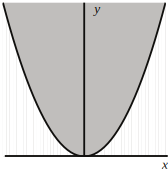
\includegraphics{figps-sec71-graph.eps}
\caption{Graph of $y \geq x^2$} \label{fig:graph-relation}
\end{center}
\end{figure}

\newpar
The points $(x, y)$ in the relation $R$ are the points on the graph of $y = x^2$ or are in the shaded region.  This because for these points, $y \geq x^2$. One of the shortcomings of this type of graph is that the graph of the equation and the shaded region are actually unbounded and so we can never show the entire graph of this relation.  However, it does allow us to see that the points in this relation are either on the parabola defined by the equation $y = x^2$ or are ``inside'' the parabola.

When the domain or range of a relation is infinite, we cannot provide a visualization of the entire relation.  However, if  $A$  is a (small) finite set, a relation  $R$  on  $A$  can be specified by simply listing all the ordered pairs in  $R$.  For example,  if  $A = \left\{ {1, 2, 3, 4} \right\}$, then 
\[
R = \left\{ {( {1, 1} ), ( {4, 4} ), ( {1, 3} ), ( {3, 2} ), ( {1, 2} ), ( {2, 1} )} \right\}
\]
is a relation  on  $A$.  A convenient way to represent such a relation is to draw a point in the plane for each of the elements of  $A$  and then for each  $\left( {x, y} \right) \in R$ (or  
$x \mathrel{R} y$),  we draw an arrow starting at the point $x$  and pointing to the point $y$.  If  
$\left( {x, x} \right) \in R$ (or  $x \mathrel{R} x$), we draw a loop at the point  $x$.  The resulting diagram is called a \textbf{directed graph} \label{directedgraph}
\index{directed graph}%
 or a \textbf{digraph}.
\index{digraph}%
  The diagram in Figure~\ref{fig:dirgraph2} is a digraph for the relation  $R$.

\begin{figure}[h]
\begin{center}
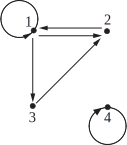
\includegraphics{figps-prev72digraph.eps}
\caption{Directed Graph for a Relation} \label{fig:dirgraph2}
\end{center}
\end{figure}

In a directed graph, the points are called the \textbf{vertices}.  So each element of  $A$  corresponds to a \textbf{vertex}.
\index{vertex}%
\index{directed graph!vertex}%
  The arrows, including the loops, are called the \textbf{directed edges}
\index{directed edge}%
\index{directed graph!directed edge}%
 of the directed graph.  We will make use of these directed graphs in the next section when we study equivalence relations.

\begin{prog}[\textbf{The Directed Graph of a Relation}]\label{prog:directedgraph} \hfill \\
Let $A = \{ 1, 2, 3, 4, 5, 6 \}$.  Draw a directed graph for the following two relations on the set $A$.  For each relation, it may be helpful to arrange the vertices of $A$ as shown in Figure~\ref{fig:dirgraph3}.
\[
R = \{ (x, y) \in A \times A \mid x \text{ divides } y \}, \qquad 
T = \{ (x, y) \in A \times A \mid x + y \text{ is even} \}.
\]
\begin{figure}[h]
\begin{center}
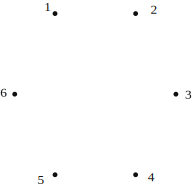
\includegraphics{figps-sec71-dirgraph.eps}
\caption{Vertices for $A$} \label{fig:dirgraph3}
\end{center}
\end{figure}
\end{prog}
\hbreak

\endinput



\endinput
Use the example in the old Preview Activity 3 as a progress check in the next subsection.

%

\subsection*{The Inverse of a Relation}
In Section~\ref{S:inversefunctions}, we introduced the \textbf{inverse of a function}.
\index{inverse of a function}%
\index{function!inverse of}%
 If  $A$ and $B$ are nonempty sets and if $f:A \to B$ is a function, then the inverse of  $f$, denoted by  $f^{ - 1} $, is defined as
\begin{align*}
f^{ - 1}  &= \left\{ { {\left( {b, a} \right) \in B \times A } \mid f\left( a \right) = b} \right\} \\
          &= \left\{ { {\left( {b, a} \right) \in B \times A } \mid \left( {a, b} \right) \in f} \right\}\!.
\end{align*}
%If we use the ordered pair representation for  $f$, we could also write
%\[
%f^{ - 1} = \left\{ { {\left( {b, a} \right) \in B \times A } \mid \left( {a, b} \right) \in f} \right\}.
%\]
Now that we know about relations, we see that  $f^{ - 1} $  is always a relation from  $B$  to 
$A$.  The concept of the inverse of a function is actually a special case of the more general concept of the inverse of a relation, which we now define.

\begin{defbox}{inverseofrelation}{Let  $R$  be a relation from the set  $A$  to the set  $B$.  The \textbf{inverse of}  $\boldsymbol{R}$,
\index{inverse of a relation}%
\index{relation!inverse of}%
 written  $R^{ - 1} $ 
\label{sym:Rinverse} and read  ``$R$  inverse,'' is the relation from  $B$  to  $A$  defined by
\[
\begin{aligned}
  R^{ - 1}  &= \left\{ { {\left( {y, x} \right) \in B \times A } \mid \left( {x, y} \right) \in R} \right\}\text{, or} \hfill \\
  R^{ - 1}  &= \left\{ { {\left( {y, x} \right) \in B \times A } \mid x \mathrel{R} y} \right\}\!. \\ 
\end{aligned} 
\]
That is, $R^{ - 1} $ is the subset of  $B \times A$ consisting of all ordered pairs  
$\left( {y, x} \right)$  such that  $x \mathrel{R} y$.}
\end{defbox}
%
\subsection*{An Example of an Inverse Relation}
Let $D$ be the ``divides'' relation on  $\mathbb{Z}$.  See Progress 
Check~\ref{prog:dividesrelation}.  So
\[
D = \left\{ { {\left( {m, n} \right) \in \mathbb{Z} \times \mathbb{Z} } \mid m\text{  divides  }n} \right\}\!.
\]
This means that we can write
%\begin{center}
$m \mid n$ if and only if $\left( {m, n} \right) \in D$.
%\end{center}
So, in this case,
\[
\begin{aligned}
D^{ - 1}  &= \left\{ { {\left( {n, m} \right) \in \mathbb{Z} \times \mathbb{Z} } \mid \left( {m, n} \right) \in D} \right\} \\ 
          &= \left\{ { {\left( {n, m} \right) \in \mathbb{Z} \times \mathbb{Z} } \mid m\text{  divides  }n} \right\}\!. \\ 
\end{aligned}
\]
Now, if we would like to focus on the first coordinate instead of the second coordinate in  
$D^{ - 1} $, we know that  ``$m$  divides  $n$''  means the same thing as  ``$n$  is a multiple of  $m$.''  Hence,
\[
D^{ - 1}  = \left\{ { {\left( {n, m} \right) \in \mathbb{Z} \times \mathbb{Z} } \mid n\text{  is a multiple of  }m} \right\}\!.
\]
We can say that the inverse of the ``divides'' relation on  $\mathbb{Z}$  is the ``is a multiple of'' relation on  $\mathbb{Z}$.
\hbreak
%
Theorem~\ref{T:inverserelations}, which follows, contains some elementary facts about inverse relations.  The proofs of these results are included in Activity~\ref{A:provinginverse}.
%
\begin{theorem} \label{T:inverserelations}
Let  $R$  be a relation from the set  $A$  to the set  $B$.  Then

\begin{enumerate}
\item The domain of  $R^{ - 1} $ is the range of  $R$.  That is, 
$\text{dom}\!\left( {R^{ - 1} } \right) = \text{range}( R )$.  \label{T:inverserelations1}

\item The range of  $R^{ - 1} $  is the domain of  $R$.   That is, 
$\text{range}\!\left( {R^{ - 1} } \right) = \text{dom}( R )$.  \label{T:inverserelations2}

\item The inverse of  $R^{ - 1} $  is  $R$.  That is, $\left( {R^{ - 1} } \right)^{ - 1}  = R$.  \label{T:inverserelations3}

\end{enumerate}
\end{theorem}
\hbreak
%
\begin{activity}[Proving Theorem \ref{T:inverserelations}] \label{A:provinginverse} \hfill \\
To prove Part~(\ref{T:inverserelations1}) of 
Theorem~\ref{T:inverserelations}, observe that the goal is to prove that two sets are equal, 
\[
\text{dom}\!\left( {R^{ - 1} } \right) = \text{range}( R )\!.
\]
One way to do this is to prove that each is a subset of the other.  Another way is to use a sequence of  ``if and only if'' statements.

To prove that  $\text{dom}\!\left( {R^{ - 1} } \right) \subseteq \text{range}( R )$, we can start by choosing an arbitrary element of  $\text{dom}\!\left( {R^{ - 1} } \right)$.  So let  
$y \in \text{dom}\!\left( {R^{ - 1} } \right)$.  The goal now is to prove that 
$y~\in~\text{range}( R )$.  What does it mean to say that  
$y \in \text{dom}\!\left( {R^{ - 1} } \right)$?  It means that there exists an  $x \in A$  such that
\[
\left( {y, x} \right) \in R^{ - 1}. 
\]
Now what does it mean to say that  $( {y, x} ) \in R^{ - 1} $?  It means that  
$( {x, y} ) \in R$.  What does this tell us about  $y$?

Complete the proof of Part~(\ref{T:inverserelations1}) of Theorem~\ref{T:inverserelations}.  Then, complete the proofs of Part~(\ref{T:inverserelations2}) and Part~(\ref{T:inverserelations3}) of Theorem~\ref{T:inverserelations}.
\end{activity}
\hbreak

\endinput


  



























